\documentclass[conference]{IEEEtran}
% \IEEEoverridecommandlockouts

\usepackage{cite}
\usepackage{amsmath,amssymb,amsfonts}
\usepackage{algorithmic}
\usepackage{graphicx}
\usepackage{textcomp}
\usepackage{xcolor}
\usepackage{tabularx}
\usepackage{array}
\usepackage{subcaption}
\usepackage{booktabs}
\usepackage{multirow}
\usepackage{hyperref}

\newcolumntype{Y}{>{\raggedright\arraybackslash}X}

\def\BibTeX{{\rm B\kern-.05em{\sc i\kern-.025em b}\kern-.08em
    T\kern-.1667em\lower.7ex\hbox{E}\kern-.125emX}}
\begin{document}

\begin{titlepage}
    \centering

    {\Huge\bfseries FES: A modular pipeline to find, encode and select relevant facts from clinical notes\par}
    \vspace{2cm}

    {\large
    A dissertation submitted in partial fulfilment of\par
    The requirement for the degree of\par
    MASTER OF SCIENCE in Artificial Intelligence\par
    in\par
    The Queen’s University of Belfast\par
    by\par
    Conor Brown\par
    4th September 2026
    }
\end{titlepage}

\title{FES: A modular pipeline to find, encode and select relevant facts from clinical notes\\}

\maketitle

\begin{abstract}
x
\end{abstract}

\begin{IEEEkeywords}
information extraction, neuro-symbolic, evidence verification, 
natural language processing
\end{IEEEkeywords}

\section{Introduction}

Epilepsy affects c. 1\% of the UK population \cite{b1} and is 
characterised by recurrent, unprovoked seizures \cite{b2}. 
Seizure frequency is a key indicator of the patient's disease
burden and is commonly used in clinical care to determine 
the appropriate treatment and as a primary outcome in 
clinical trials. Despite the critical role of this information, the 
only place it is routinely recorded is in clinic letters. Clinic 
letters are unstructured narrative reports of a patient's
recent visit to the epilepsy clinic, and they often 
combine descriptions of past diagnoses, current symptoms 
and future treatment. This information can be used to 
conduct retrospective studies or to identify patient cohorts 
for clinical trials, but extracting it into that structured form 
requires experts to conduct costly, error-prone manual 
chart review. 

Natural language processing (NLP) has been used to 
automatically extract key information from clinic letters. 
Rules-based methods successfully extracted structured 
facts about medications and diagnoses, but struggled
with the imprecise language and diverse forms of seizure 
frequency statements \cite{b3}. '2 to 3 seizures a week', 
'frequent bouts of seizures' and '4 since her last visit' are 
all valid descriptions of the same fact, but designing 
rules to accommodate these completely and consistently
is very time-consuming and challenging. Rules-based 
methods are highly valued by clinicians because they
produce highly interpretable results and can flexibly 
incorporate local domain expertise, but a different
kind of tool is needed for these semantically complex 
tasks.

Large language models (LLMs) have emerged as a 
powerful tool and perform significantly better on semantically
complex tasks, including seizure frequency extraction \cite{b4}. 
However, unlike rules-based methods the outputs of 
LLMs are not constrained to the exact text they were
given and this presents challenges for the task of 
information extraction (IE). When given the specific 
task of estimating a patient's seizure frequency from 
the provided clinic letter, an LLM occasionally provided 
diagnostic advice including prescriptions for the epilepsy 
patients. This phenomenon of 'hallucination' has been
documented as a common error mode for LLMs and
is a significant risk when used to produce clinical 
information at scale. Fine-tuning an LLM on the task 
minimises this error but requires substantial training data
and computational resources. 

Prior work has utilised rules as a light post-processing
layer to repair malformed outputs from LLMs \cite{b5}, but 
none examine a hybrid pipeline of LLM and rules as a cheaper alternative to 
fine-tuning LLMs. Rules are very effective at processing 
information in a transparent, logical, configurable way. 
LLMs are very effective at extracting rich information from
semantically dense sources. Leveraging both capabilities
at distinct stages can combat the concerns about LLMs
being a black that produces hallucinations, while providing
greater semantic depth with significantly less time spent
developing rules. A combination of LLMs and rules could 
produce a more transparent, flexible system.

Effective IE can be broken down into three key stages: 
finding relevant candidate facts, encoding those facts into 
a particular form, and selecting which facts to keep and 
which to filter out. A clinic letter can describe multiple 
seizure events with varying degrees of precision 
on different occasions. Frequencies can be expressed as a 
rate, a vague quantity or a duration. Deciding which of 
those facts to preserve and how to represent them is a 
subjective clinical policy. The same evidence can be 
interpreted differently by different clinicians or presented 
in multiple forms for distinct use cases. A flexible system 
would recognise this key feature of clinical information 
and make information available for reuse across multiple 
scenarios. A transparent system would allow users to 
see the final answer and the steps taken to determine it. 

This paper evaluates the performance of LLMs and 
rules across those three stages: find, encode and select. 
It was evaluated on a set of 1,200 epilepsy clinic letters 
with a single seizure frequency label per letter annotated
by experts. A direct comparison to Gan \emph{et. al}\cite{b3} 
demonstrates that a modular system combining LLMs and 
rules with can deliver accuracy comparable to a fine-tuned 
LLM while preserving a richer chain of evidence. The 
system is available as an open source package \href{https://github.com/cbrown564-alt/clinical_extraction}{here} 
along with a web app demonstrating key features of
the pipeline \href{https://clinical-extraction.vercel.app/workbench}{here} .

\section{Literature Review}

The best approach to extract seizure frequency 
information from epilepsy clinic letters is an active area 
of research, with experiments using rules-based methods \cite{b4, b6}, 
transformers-based methods \cite{b3, b5, b7, b8} and a 
combination of both \cite{b9, b10} all published this decade. 
Rules-based methods struggled with the 
lexical variety of seizure frequency descriptions. A key 
challenge with both rules-based methods and BERT-based 
methods was their failure to generalise to letters from a 
different hospital. \cite{b6, b10}. LLMs were the first method
to demonstrate strong generalisation to a new dataset\cite{b3},
but this was achieved by fine-tuning a model on over 1,000
synthetic letters. This paper explores whether similar
performance can be achieved without any additional 
training or fine-tuning.

Rules have been used as a form of minimal post-processing 
to repair malformed outputs from LLMs \cite{b5}, but none of 
the research has explored whether a hybrid pipeline combining 
an LLM and rules at distinct stages can achieve superior 
performance than either component alone. Rules were used 
to normalise frequencies and dates as a separate layer in two
BERT-based pipelines \cite{b9, b10}, but this has not been 
replicated yet for modern LLMs. Both BERT and LLMs are 
based on the same underlying transformers architecture, but
LLMs are distinguished primarily by the fact they are trained
on massive datasets with massive parameter counts which 
led to the emergent capability of in-context learning\cite{b11}.
This capability has been shown to transfer to clinical information
extraction among many other domains, and it has been shown
that giving the LLM clear instructions and examples can replace
the need for complex post-processing\cite{b12}. This paper 
explores whether LLM instructions and examples can be 
combined with complex post-processing to replace the need 
for fine-tuning.

Clinical IE has been defined as the automatic extraction 
and encoding of clinical information from text \cite{b13}, 
composed of the two distinct tasks named entity recognition 
(NER) and concept encoding \cite{b14}. Despite this, the
seizure frequency extraction pipelines using LLMs bundle 
both tasks into a single step by asking the model to output 
a normalised label e.g. '4 per month' from a raw statement 
'about once a week'. A third task exists in many clinical 
extraction pipelines but goes unmentioned: selection. This
was a distinct stage in prior rules-based systems\cite{b15} but is
bundled into a single LLM prompt with the two other tasks. In 
a clinic letter with multiple seizure frequency statements,
if the task is to output a single label describing the patient's
current seizure frequency burden, the task contains
three components. The model needs to find relevant 
seizure frequency statements in the text, encode them 
into a normalised form and select the one that best 
answers the question. This paper explores whether defining
find, encode and select as separate stages in a modular 
pipeline can deliver comparable performance while 
preserving more of the evidence for downstream use.

Academic papers tend to focus exclusively on benchmark 
accuracy while practitioners tend to value transparency, 
configurability and efficiency at the cost of some accuracy\cite{b15}. 
Model interpretability is also a critical factor clinical settings\cite{b14}. 
Clinicians are trained to use deductive logic to draw 
conclusions and they expect systems to expose transparent, 
interpretable evidence that they can reliably use to make 
decisions that demand high accountability. Past work 
utilises evidence spans as a training input\cite{b3} for 
fine-tuning or as data exhaust as part of using a rule-based 
method{b4}. This paper explores whether preserving a 
transparent evidence chain from exact text to final answer 
can make the output both more interpretable and more 
accurate.

\section{Methods}
\subsection{Data}

The dataset is a collection of epilepsy clinic letters which 
record a UK patient's consultation with an epilepsy 
specialist, often a neurologist or specialist nurse \cite{b3} 
The NHS requires that clinic letters are sent to the 
patient's GP after all outpatient visits such as these.
They are often the only record of a patient's diagnoses,
treatments and outcomes in neurological disorders, 
and they are written in narrative form. An example clinic letter 
is shown in Figure~\ref{letter}.

\begin{figure}[t]
    \centering

    
\includegraphics[width=\linewidth]{example_clinic_letter.png}
    \caption{An example clinic letter with two distinct seizure frequency statements highlighted as potential candidates.}
    \label{letter}
\end{figure}

Gan \emph{et al.}\cite{b3}  produced this dataset of synthetic 
letters modelled on real clinic letters from King's College 
London hospital. The real letters were used to create 10 
template letters and they were combined with 500 short 
descriptions of seizure frequency statements produced 
by GPT-5 to create the full set of 15,099 letters. A sample 
of 1,200 letters was used in this paper. Each seizure 
frequency statement was annotated by trained experts 
to create the gold-standard labels. Each letter has a 
single label representing the patient's current seizure 
frequency burden.

\begin{table}[!t]
\caption{Dataset summary}
\label{tab:dataset}
\centering
\begin{tabularx}{\linewidth}{lYcc}
\toprule
 & & \textbf{Development} & \textbf{Test} \\
\midrule
\multicolumn{2}{l}{Number of letters} & 750 & 450 \\
\midrule
\multirow{4}{*}{Seizure frequency} & Frequent & 51\% & 50\% \\
 & Infrequent & 17\% & 18\% \\
 & Unknown & 17\% & 17\% \\
 & Seizure free & 15\% & 15\% \\
\bottomrule
\end{tabularx}
\end{table}

Minimal preprocessing was applied to the raw data.
Letters and annotations were stored in a single 
.json file. Letters are minimally cleaned to correctly 
parse quotes, new lines, tabs, the $\leq$ sign and 
nulls. The raw letters were ingested in the pipeline 
in full; no tokenisation, section-splitting or truncation 
was applied. 

The dataset was split into a development set of 750
letters and a test set of 450 letters, stratified by their 
seizure frequency category (frequent, infrequent, 
unknown, seizure free) to balance the distribution 
across both splits. The exact breakdown can be 
seen in Table~\ref{tab:dataset}.

\subsection{Architecture}

The pipeline is divided into three key stages: find,
encode, select. First, the pipeline finds seizure frequency
events that fit the description in the raw text. Next, the 
pipeline takes the raw text from those candidates and 
encodes them into a normalised form. Finally, the pipeline 
selects the final answer from the set of candidate facts,
either combining them together or choosing one. Figure~\ref{pipeline}
illustrates the architecture of the pipeline with a real 
example from the development set.

This paper evaluates three main methods on this 
pipeline: \texttt{Rules only}, \texttt{LLM only}, and \texttt{LLM and Rules}. 
Table~\ref{tab:method} summarises their configuration
at each stage. \texttt{Rules only} and \texttt{LLM only} serve as the 
baselines to illustrate how effectively each method performs in isolation. 
\texttt{LLM and Rules} illustrates 
the ideal combination of the two: the LLM finds and
encodes relevant seizure frequency events, then rules 
are layered on top to encode and select the final 
answer. The LLM prompt design and rule design 
sections below describe the implementation details.
The combined \texttt{LLM and Rules} method could
be configured in multiple other ways, but this is the
optimal combination. Further configurations are 
described and evaluated in the results sections.

\begin{figure*}[t]
    \centering

    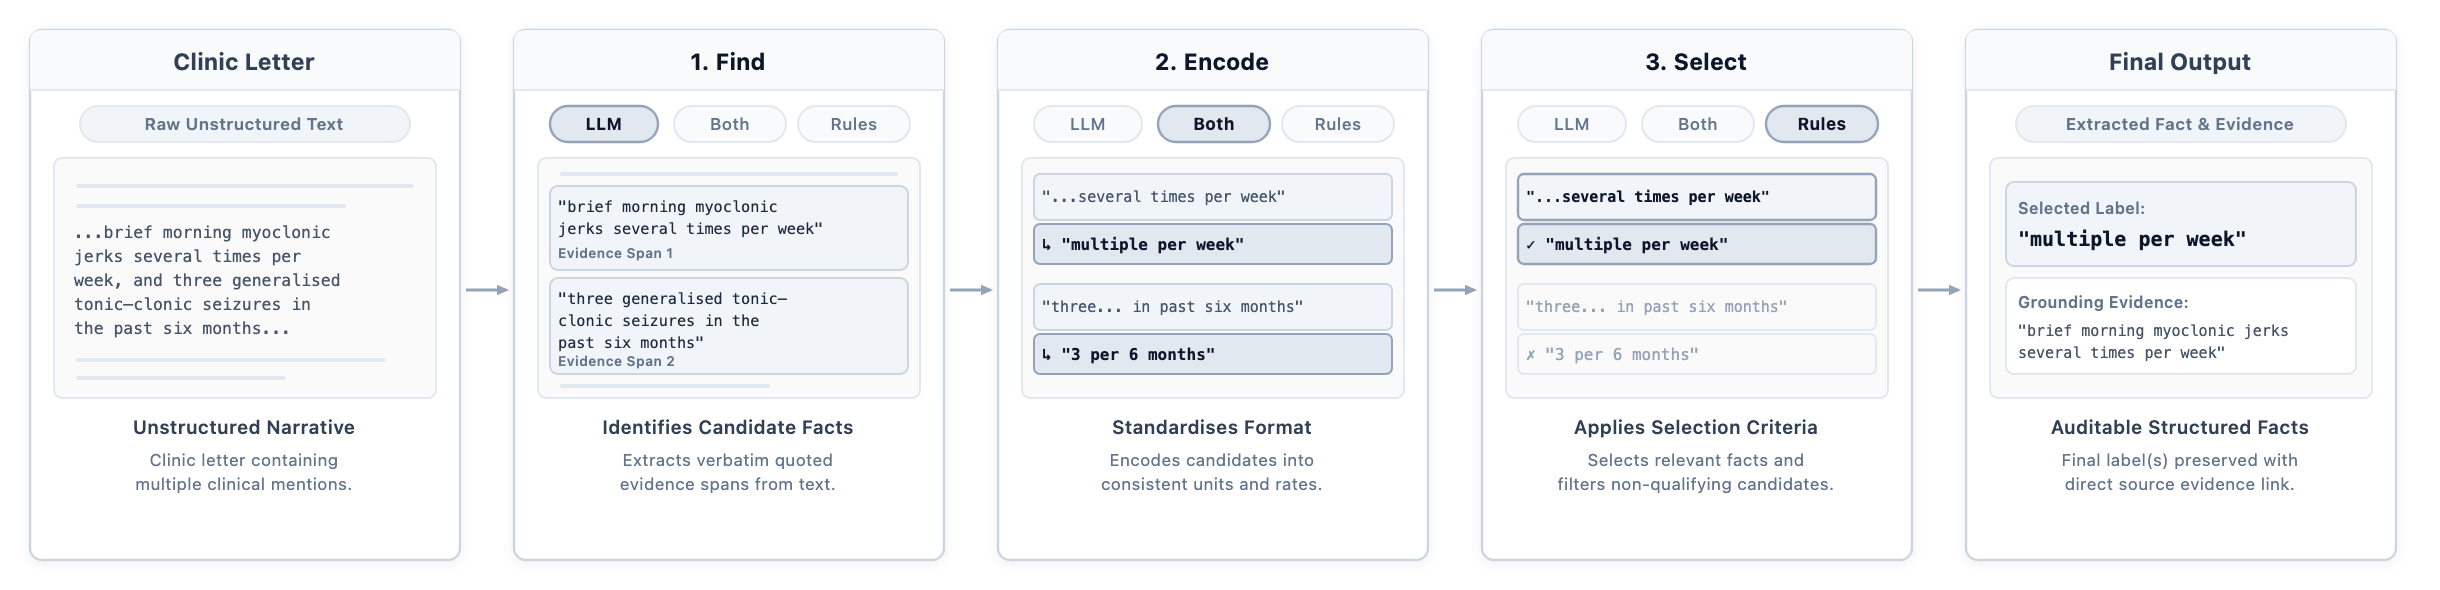
\includegraphics[width=\linewidth]{pipeline_architecture.png}
    \caption{A clinic letter passes through three stages in the pipeline - find, encode and select - to generate structured labels with the exact text used from the letter to produce the label. Each of the three stages can be configured to use an LLM, rules or both. The example shown is the task of extracting a single label representing the patient's current seizure frequency burden.}
    \label{pipeline}
\end{figure*}

\begin{table}[!t]
\caption{Method configuration by pipeline stage}
\label{tab:method}
\centering
\begin{tabularx}{\linewidth}{Ylll}
\toprule
\textbf{Method} & \textbf{Find} & \textbf{Encode} & \textbf{Select} \\
\midrule
Rules only & Rules & Rules & Rules \\
LLM and Rules & LLM & LLM and Rules & Rules \\
LLM only & {LLM$^\ast$} & & LLM \\
\bottomrule
\end{tabularx}

\vspace*{2pt}
\begin{minipage}{\linewidth}
\raggedright\footnotesize
$^\ast$A single LLM prompt is used for the find and encode stages. A second LLM prompt is used for select. 
\end{minipage}
\end{table}

\subsection{LLM Prompt Design}

The most consequential component of the \texttt{LLM and Rules}
and \texttt{LLM only} methods is the single prompt used for the
find and encode stages. It is composed of three main 
elements: 
\begin{enumerate}
\item Instructions to identify relevant seizure 
frequency facts at the appropriate granularity
\item Examples of how the seizure frequency facts should
be represented
\item The schema to represent them in
\end{enumerate}

A key design choice in this pipeline is to represent multiple 
seizure frequency events with exact evidence to enable 
a subsequent LLM call or rules to review that evidence 
and refine the final answer. The model finds multiple 
candidate events and selects the best candidate, but that
answer can be updated.

Key instructions include: 

\begin{enumerate}
\item When several current seizure types are present, 
select the highest current or recent burden
\item When the letter gives an overall current count and 
a breakdown by type, select the overall count
\item Use \texttt{no\_reference} only when the letter has 
no usable seizure frequency evidence, and use
\texttt{unknown\_frequency} when seizures are discussed 
but frequency is unclear
\item Keep seizure-free statements separate from unknown 
or last-event statements, and do not select seizure-free if 
other current seizure-like events 
remain active
\end{enumerate}

The model is instructed to assign each event to one of 
the six categories described in Table~\ref{tab:event-categories}
and assign a label to each event in one of the forms 
represented in (Table~\ref{tab:label-forms}). 

\begin{table}[!t]
\caption{Find event categories}
\label{tab:event-categories}
\centering
\begin{tabularx}{\linewidth}{lY}
\toprule
\textbf{Category} & \textbf{Use} \\
\midrule
\texttt{frequency\_rate} & A countable or range rate \\
\texttt{cluster\_frequency} & How often clusters occur \\
\texttt{seizure\_free} & A seizure-free statement \\
\texttt{last\_event\_only} & A dated last event without a rate \\
\texttt{unknown\_frequency} & Seizures discussed, no usable rate \\
\texttt{no\_reference} & No usable frequency evidence \\
\bottomrule
\end{tabularx}
\end{table}

\begin{table}[!t]
\caption{Seizure-frequency label forms}
\label{tab:label-forms}
\centering
\begin{tabularx}{\linewidth}{lY}
\toprule
\textbf{Family} & \textbf{Written forms} \\
\midrule
Rate &
$N$ per unit;
$N$ per $N$ unit;
$N$ per $N$ to $N$ unit;
$N$ to $N$ per unit;
$N$ to $N$ per $N$ unit;
multiple per unit;
multiple per $N$ unit;
$N$ per multiple unit \\
Cluster &
cluster per unit, $N$ per cluster;
cluster per unit, range per cluster;
cluster per unit, multiple per cluster;
unknown cluster count \\
Seizure free &
seizure free for a duration;
seizure free for a vague duration \\
Sentinel &
unknown;
no seizure frequency reference \\
\bottomrule
\end{tabularx}
\end{table}

\subsection{Rule Design}


\subsection{Pipeline Optimisation}

The development set was used to optimise the two key 
elements of the pipeline: the LLM prompt instructions and 
the rules. The focus of the optimisation process was to 
improve accuracy while keeping the instructions and rules 
simple and generalisable. Qualitative error analysis was 
conducted to diagnose the cause of poor performance 
in particular areas and identify common error modes. 
Hypotheses were developed and tested to tune the 
prompt and rules iteratively. 

Through iterative error analysis on both the LLM and 
the rules, it became apparent that the complexity of the 
task was often a function of competing rules and 
guidelines. Often, improving a rule or a prompt 
instruction to address one class of error would harm 
another area because annotation policies are complex.
This complexity is a challenge for human annotators 
also; Fonferko-Shadrach \emph{et al.} described seizure
frequency as the most difficult category to annotate
and their inter-annotator agreement of 0.47 shows 
annotators often disagreed about how to represent
seizure frequency statements\cite{b4}.

Decomposing the task into three stages allowed for 
cleaner separation of the policies on which types of 
facts to extract and which criteria to apply to exclude
specific variants of them. Decomposing the task into
three stages also made it possible to evaluate the 
performance at each individual stage and identify the 
bottlenecks in the system. It is this combination of 
a cleaner task decomposition for the pipeline and a
clearer view into the pipeline that enabled steady,
incremental gains to materialise from the optimisation
process.

\subsection{Evaluation}

To enable a direct comparison with the results in 
Gan \emph{et. al}, the pipeline is evaluated using the 
same micro-F1 score. They calculate the F1 on two 
categories; a fine-grained \texttt{purist} score and a 
coarser '\texttt{pragmatic}' score. The more precise
\texttt{purist} F1 is the primary metric in this paper, 
but \texttt{pragmatic} F1 is used for frequency bands 
with very small sample sizes (\textless20). A full 
specification of the categories is in Table~\ref{tab:categories}. 
The rationale for categorising labels is so that 
semantically identical phrases are matched when 
exact labels differ; so that daily, once per day and 
every day would be considered correct matches 
to the gold label '1 per day'. This evaluates the model 
on how effectively it can identify the correct frequency 
rather than replicate precise phrasing. Further 
explanation on the categories can be found in the 
original paper from Holgate \emph{et. al}\cite{b5}.

The pipeline is evaluated on a held-out test set of 450 
letters.These letters were never used to tune prompts, 
rules or any other aspect of the pipeline. The test set is 
therefore used to evaluate how effectively the model 
generalises to unseen data. These results are compared 
against the evaluation set labelled Synthetic (1,166) in 
Gan \emph{et. al}\cite{b3} which was also a held-out 
sample from the synthetic dataset, distinct from the 
training set used to fine-tune the models. 

\begin{table}[!t]
\caption{Seizure frequency categories: Purist and Pragmatic}
\label{tab:categories}
\centering
\begin{tabularx}{\linewidth}{Yl}
\toprule
\textbf{Purist} &
\textbf{Pragmatic} \\
\midrule
Daily & \multirow{4}{*}{Frequent} \\
More than weekly, less than daily & \\
Once a week & \\
More than monthly, less than weekly & \\
\midrule
Once a month & \multirow{4}{*}{Infrequent} \\
More than every 6 months, less than monthly & \\
Once every 6 months & \\
Less than once every 6 months & \\
\midrule
Unknown & Unknown \\
\midrule
Seizure free & Seizure free \\
\bottomrule
\end{tabularx}
\end{table}

The primary objective of this research is to assess whether
a combination of an LLM and rules perform better than 
their individual component parts. The secondary objective 
is to identify which component performs best at which stage. 
Table~\ref{tab:method} shows the 3 methods used in the 
evaluation: \texttt{Rules only}, \texttt{LLM only} or a 
combination of \texttt{LLM and Rules}. Each method was 
evaluated at each stage: find, encode and select. This 
produces a 3x3 matrix of results 
that answer two key questions: 

\begin{enumerate}
\item Among the three methods, which performs
best: rules, LLM, or a combination of both?
\item How much incremental value is there from the additional
encode and select stages?
\end{enumerate}

The primary hypothesis is that a combination of an LLM
plus rules will perform better than either on their own, 
because they have complementary strengths and those 
strengths are particularly well suited to distinct stages in
the pipeline. The secondary hypothesis is that multiple 
discrete stages will improve performance for the LLM,
regardless of whether the subsequent stages are rules or 
additional LLM calls. This builds on the idea that task 
decomposition is an effective form of context engineering, 
and is particularly useful in scenarios where the prompt 
is long and contains many layers of instructions. 

\section{Results}

\subsection{Benchmark Performance}

FIRST PARAGRAPH NEEDS TO SUMMARISE THE APPROACH TO THE PROBLEM (DATA, EVALUATION) AND NOVEL METHOD CONTRIBUTIONS

The \texttt{LLM and Rules} method achieves state-of-the-art results
(SOTA) for extracting seizure frequency from epilepsy letters.
It achieved a \texttt{purist} micro-F1 score of 0.86, exceeding the 
prior benchmark performance of 0.81 in Gan \emph{et. al} 
set by a model that was fine-tuned and evaluated using 
this same dataset of synthetic letters. While that is the only
paper to evaluate the same dataset with the same metric, 
Table~\ref{tab:historical} includes a summary of all 7 papers that reported 
a seizure frequency extraction score this decade.  

\begin{table}[!t]
\caption{Comparisons to past seizure frequency papers}
\label{tab:historical}
\centering
\begin{tabularx}{\linewidth}{Ycll}
\toprule
\textbf{Author} & \textbf{Year} & \textbf{Method} & \textbf{F1 score} \\
\midrule
Xie et al. & 2022 & Fine-tuned BERT & 0.83$^\ast$ \\
Decker et al. & 2022 & Rules & 0.82$^\ast$$^\ast$ \\
Fonferko-Shadrach et al. & 2024 & Rules & 0.66 \\
Fernandes et al. & 2024 & Fine-tuned BERT & 0.37 \\
Holgate et al. & 2024 & Prompted LLM & 0.73 \\
Holgate et al. & 2025 & Fine-tuned LLM & 0.68 \\
Gan et al. & 2026 & Fine-tuned LLM & 0.81 \\
\midrule
Brown \& Gan & 2026 & LLM and rules & 0.86 \\
\bottomrule
\end{tabularx}

\vspace*{2pt}
\begin{minipage}{\linewidth}
\raggedright\footnotesize
$^\ast$Drops to 0.73 on texts with a frequency statement.
\end{minipage}

\begin{minipage}{\linewidth}
\raggedright\footnotesize
$^\ast$$^\ast$Drops to 0.4 on the external test set. 
\end{minipage}
\end{table}

This method is particularly effective at identifying 
countable rates, including high-frequency events. A common theme in 
previous papers is that their method performed 
best when the task was predicting  '\texttt{unknown}' or  
\texttt{no seizures}. Xie et. al reported an F1 score of 0.92 on 
texts that contained no seizure frequency statement and 
0.73 when there was a seizure frequency reported. Gan 
et al. and Holgate et. al both report \texttt{unknown} as their 
highest scoring category at 0.89 and 0.87 respectively, 
while \texttt{daily} (0.7, 0.41) and \texttt{more than weekly} 
(0.68, 0.55) are much lower. In this method, \texttt{daily} (0.92) and 
\texttt{more than weekly} (0.91) are among the best performing 
categories, significantly above \texttt{unknown} (0.74). The full
performance breakdown across \texttt{purist} and \texttt{pragmatic} 
categories can be seen in Table~\ref{tab:performance}.

\begin{table}[!t]
\caption{LLM and Rules: Purist and Pragmatic micro-F1}
\label{tab:performance}
\centering
\begin{tabularx}{\linewidth}{Yccc}
\toprule
\textbf{Purist} &
\textbf{\emph{n}} &
\textbf{Purist F1} &
\textbf{Pragmatic F1} \\
\midrule
Daily & 41 & 0.92 & \multirow{4}{*}{Frequent: 0.95} \\
More than weekly, less than daily & 123 & 0.91 & \\
\textcolor{black!55}{Once a week} & \textcolor{black!55}{5} & \textcolor{black!55}{0.89} & \\
More than monthly, less than weekly & 58 & 0.90 & \\
\midrule
Once a month & 18 & 0.94 & \multirow{4}{*}{Infrequent: 0.82} \\
More than every 6 months, less than monthly & 55 & 0.81 & \\
\textcolor{black!55}{Once every 6 months} & \textcolor{black!55}{1} & \textcolor{black!55}{0.00} & \\
\textcolor{black!55}{Less than once every 6 months} & \textcolor{black!55}{6} & \textcolor{black!55}{0.60} & \\
\midrule
Unknown & 76 & 0.74 & Unknown: 0.74 \\
\midrule
Seizure free & 67 & 0.90 & Seizure free: 0.90 \\
\bottomrule
\end{tabularx}

\vspace*{2pt}
\begin{minipage}{\linewidth}
\raggedright\footnotesize
Rows with $n{<}10$ shown in grey.
\end{minipage}
\end{table}

\subsection{Method Performance by Stage}

The \texttt{LLM and Rules} method performs better than the LLM or 
rules alone at every stage: find, encode, select  (Table~\ref{tab:stages}).
The LLM is significantly better at at the initial find
stage vs. rules alone (0.79 vs 0.65). The \texttt{LLM and Rules} 
combination then adds incremental gains at the encode 
(+0.01) and select (+0.06) stages, while the subsequent
LLM stages make a very marginal difference (+0.006). 
This illustrates that the LLM and rules have complementary 
strengths that are particularly effective at discrete stages.

The LLM is particularly strong at the find stage: 
identifying high quality candidates in the text and 
providing an initial proposed answer in the required form. 
This initial stage is equivalent to the entire extraction 
pipeline in most prior papers: find, encode and 
select all at once. The LLM at this stage performs at
a level comparable to the best prior methods, achieving
performance in a single prompt that previously required 
fine-tuning. 

Rules are particularly effective at the select stage: 
reviewing all of the candidates proposed by the model
and determining which should be the final answer. 
This can mean either choosing a different candidate, 
such as choosing a frequency candidate when the model 
has chosen \texttt{unknown}, or performing a mathematical 
calculation on the selected evidence to update the answer,
such as counting the total events over a monthly seizure 
diary. This is a direct consequent of the pipeline design. 
The find phase outputs multiple candidate events with 
evidence quoted directly from the text, rather than just a 
single flat answer. Rules leverage that richer evidence to 
deliver significant incremental gains.

\begin{table}[!t]
\caption{Purist micro-F1 at find, encode, and select}
\label{tab:stages}
\centering
\begin{tabularx}{\linewidth}{Ylll}
\toprule
\textbf{Method} &
\textbf{Find} &
\textbf{Encode} &
\textbf{Select} \\
\midrule
Rules only & 0.65 & 0.65 & 0.72 \\
LLM + rules & 0.79 & 0.80 & 0.86 \\
LLM only & \multicolumn{2}{c}{0.79$^\ast$} & 0.79 \\
\bottomrule
\end{tabularx}

\vspace*{2pt}
\begin{minipage}{\linewidth}
\raggedright\footnotesize
$^\ast$A single LLM prompt is used for the find and encode stages.
\end{minipage}
\end{table}

\subsection{Model Comparison}

The \texttt{LLM and Rules} method shows consistent, 
incremental performance gains on each of the six
models evaluated (Figure~\ref{models}). The 
average performance gain was +0.07 from find
to select, with Luna showing the largest gain of 
+0.10. Model performance on \texttt{purist} F1 closely 
correlates to overall medical intelligence as 
measured by Artificial Analysis' Healthcare and 
Medical Index. They cluster into three groups:
strong (Gemini 0.86, Grok 0.85), medium (DeepSeek
0.82, Luna 0.79), weak (Qwen 0.76, Gemma 0.72)
which largely reflect the model size and cost.

Local models that fit on consumer-grade hardware
now deliver superior performance to models that
required eight Nvidia V100 GPUs two years ago 
(Holgate, 2024). Qwen's performance of 0.76 was 
achieved running locally on a laptop with a single
GPU, surpassing Llama 2's performance of 0.73. 
That is a critical development as it means hospitals 
can use their own servers to securely process patient 
data to reliably extract clinical information like this. 
DeepSeek is small enough for many hospital servers
to host and it performs better than a model fine-tuned
on 1,797 synthetic letters. 

\begin{figure}[t]
    \centering

    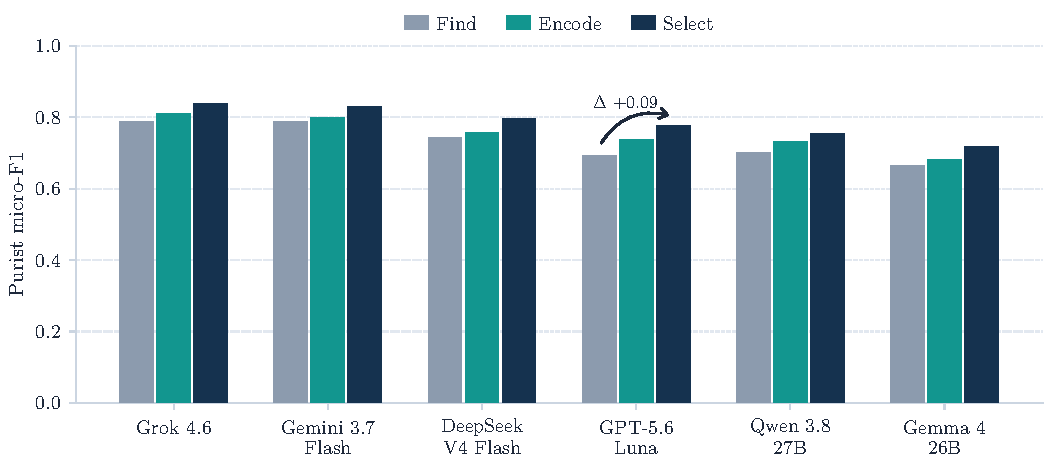
\includegraphics[width=\linewidth]{six_model_stage_performance.pdf}
    \caption{LLM and rules. Every model sees consistent performance gains in the encode and select stages. Luna saw the biggest performance gain (0.69→0.79).}
    \label{models}
\end{figure}

\begin{figure}[t]
    \centering

    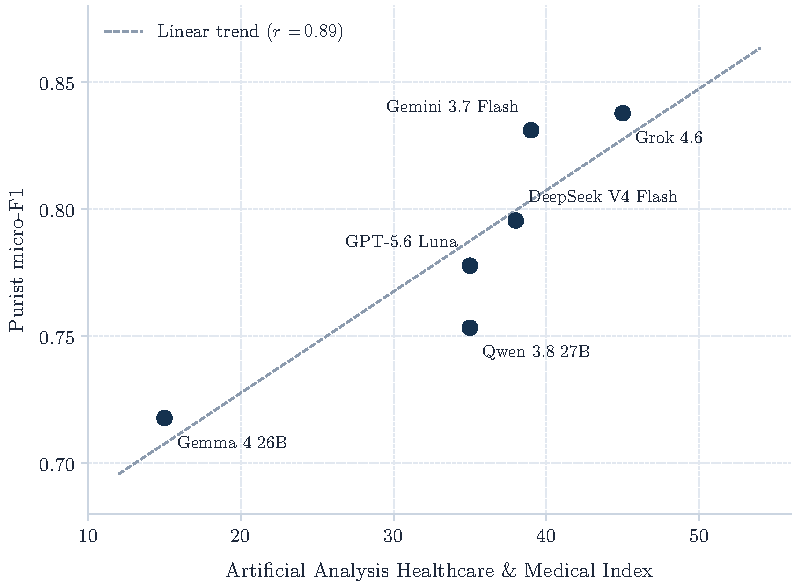
\includegraphics[width=\linewidth]{healthcare_index_vs_purist_f1.pdf}
    \caption{The smartest models are the best frequency extractors.}
    \label{models}
\end{figure}

\subsection{Model Configuration}

Raising the reasoning effort level did not improve 
performance. Gemini's \texttt{purist}-F1 score was 0.86 at low and 
0.84 at high; a paired difference of +0.02, 95\% CI -0.01 to 
0.04; p = 0.31. Extra reasoning adds cost and latency without 
improving extraction.

The temperature setting also had no significant effect on the
results. The F1 score was 0.86 on a temperature of 0 versus 
0.84 at a temperature of 1 (paired difference +0.02, 95\% CI 
-0.01 to 0.04; p = 0.20).  A temperature of 0 was an appropriate
default across models and Luna at a temperature of 1 is a 
valid comparison.

The task is tightly defined with explicit schema and output 
requirements, which limits the expected variability by design.
This partly explains why neither setting had a significant effect 
on results and it indicates the robustness of the method.

\subsection{Development vs. Test Results}

\texttt{Rules only} perform better on the development set but 
significantly worse on the test set (Figure~\ref{devtest}), which 
repeats the pattern of overfitting commonly found in the literature. 
Rules are brittle and tend to overfit specific patterns in the 
training data, generalising poorly to unseen data. The \texttt{Rules
only} method achieves an F1 score of 0.92 on the 
development set, but performance declines significantly 
(-0.20) on the test set. \texttt{LLM only} achieves a consistent score of 0.79 
across both splits which shows the method generalises 
well. The \texttt{LLM and Rules} method combines the best parts of each:
it performs significantly better on the development set than LLM
only (+0.08) and it has a significantly smaller generalisation gap
than rules only (-0.01). The LLM does the heavy lifting 
of matching patterns across the entire text, allowing the
rules to focus on generalisable patterns in the refined 
evidence set.

\begin{figure}[t]
    \centering

    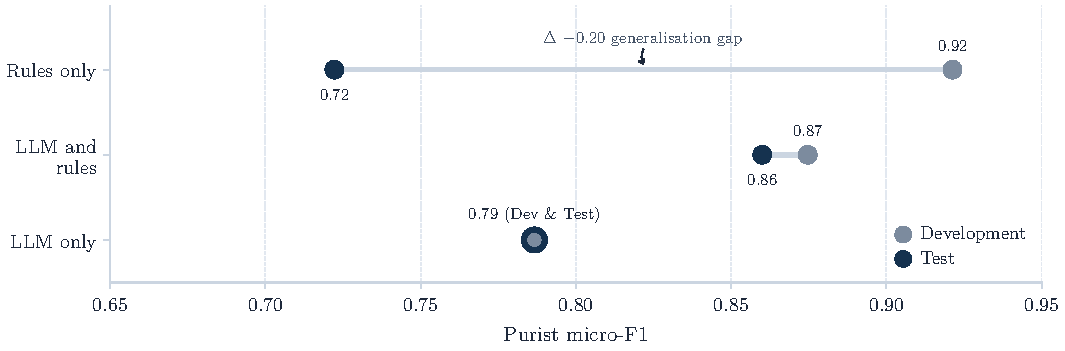
\includegraphics[width=\linewidth]{development_vs_test_generalization.pdf}
     \caption{Rules only performs best on the development set but overfit. LLM only generalises best with consistent performance. LLM and rules combined produce the best results overall, even with a generalisation gap of -0.01 (0.87→0.86).}
    \label{devtest}
\end{figure}

\subsection{Error Analysis}

The worst performing category was \texttt{unknown} with an F1 
score of 0.74. 69\% of the errors (37/54) are incorrect
selections of \texttt{unknown}. The full error distribution is shown 
in the confusion matrix (Figure~\ref{confusion}). 

Illustrative examples of the three most common errors - \texttt{infrequent → 
unknown} (16), \texttt{frequent → unknown} (13), and \texttt{seizure free →
unknown} (8) - are shown in Figure~\ref{errors}. The errors
reflect a cautious approach when the evidence is ambiguous,
for example the model recognised the phrase 'these episodes
crop up most shifts' as the primary seizure frequency 
description but refused to make an assumption about how
many shifts the person has. This cautious assessment is 
justifiable and a key benefit of this method is the exact 
evidence is preserved, so any downstream users can see 
the proposed answer while also drawing their own conclusion
from the neatly packaged evidence.

\begin{figure}[t]
    \centering

    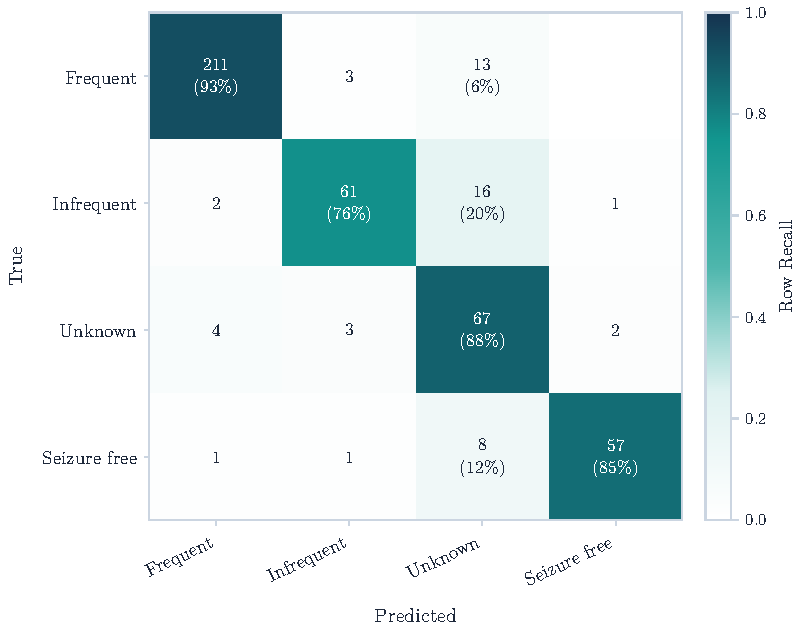
\includegraphics[width=\linewidth]{confusion_matrix_pragmatic.pdf}
     \caption{Unknown was the category with the most incorrect predictions from all 3 categories.}
    \label{confusion}
\end{figure}

\begin{figure*}[t]
    \centering
    \begin{subfigure}[t]{\linewidth}
        \centering
        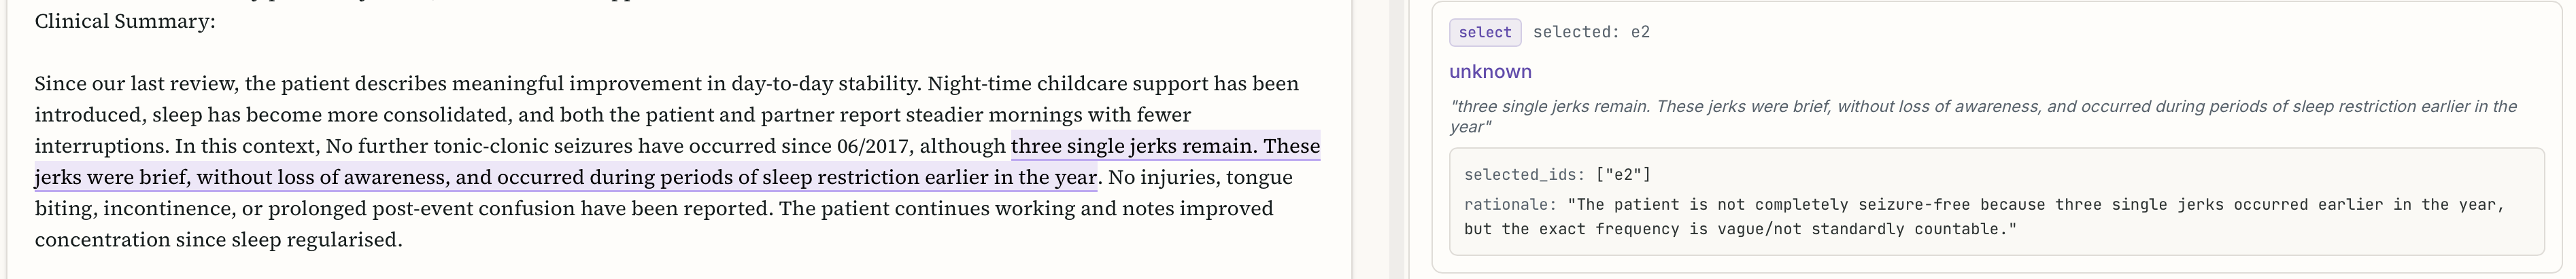
\includegraphics[width=\linewidth]{infrequent_unknown1.png}
        \caption{Infrequent → unknown error example. Gold-standard label: 3 per 14 month. Model selected unknown. }
        \label{fig:infrequent_unknown1}
    \end{subfigure}
    \vspace*{4pt}
    \vspace*{4pt}
    \begin{subfigure}[t]{\linewidth}
        \centering
        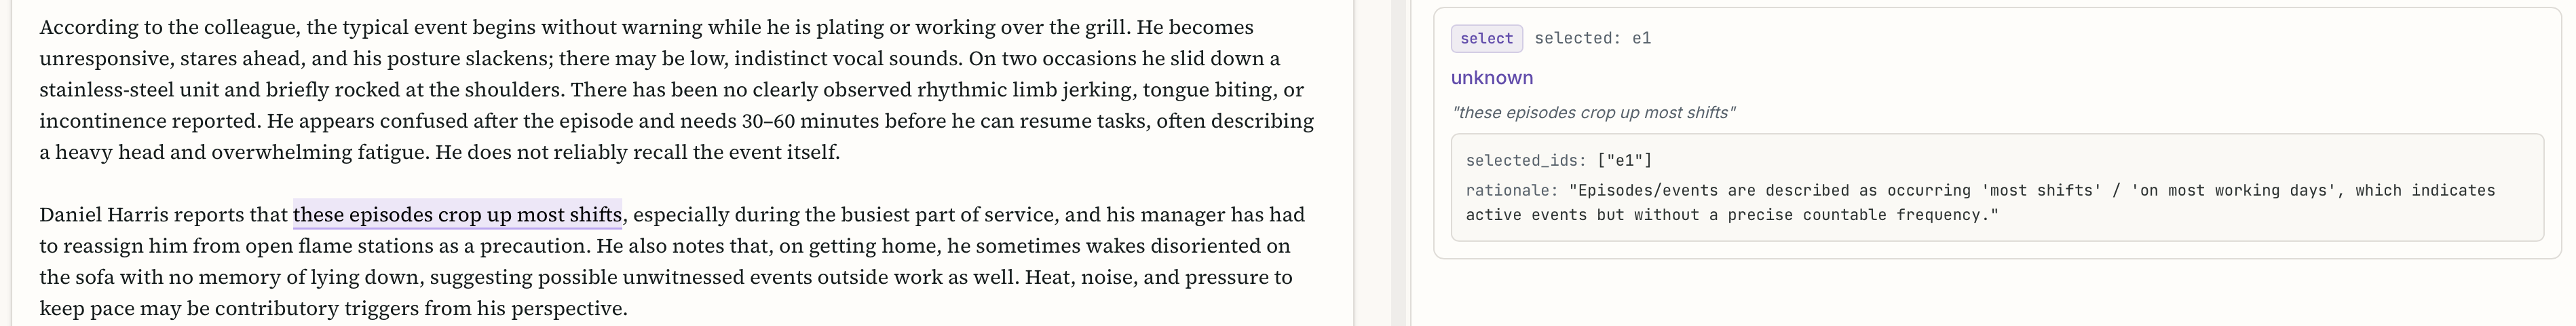
\includegraphics[width=\linewidth]{frequent_unknown1}
        \caption{Frequent → unknown error example. Gold-standard label: multiple per week. Model selected unknown.}
        \label{fig:frequent_unknown1}
    \end{subfigure}
    \vspace*{4pt}
    \vspace*{4pt}
    \begin{subfigure}[t]{\linewidth}
        \centering
        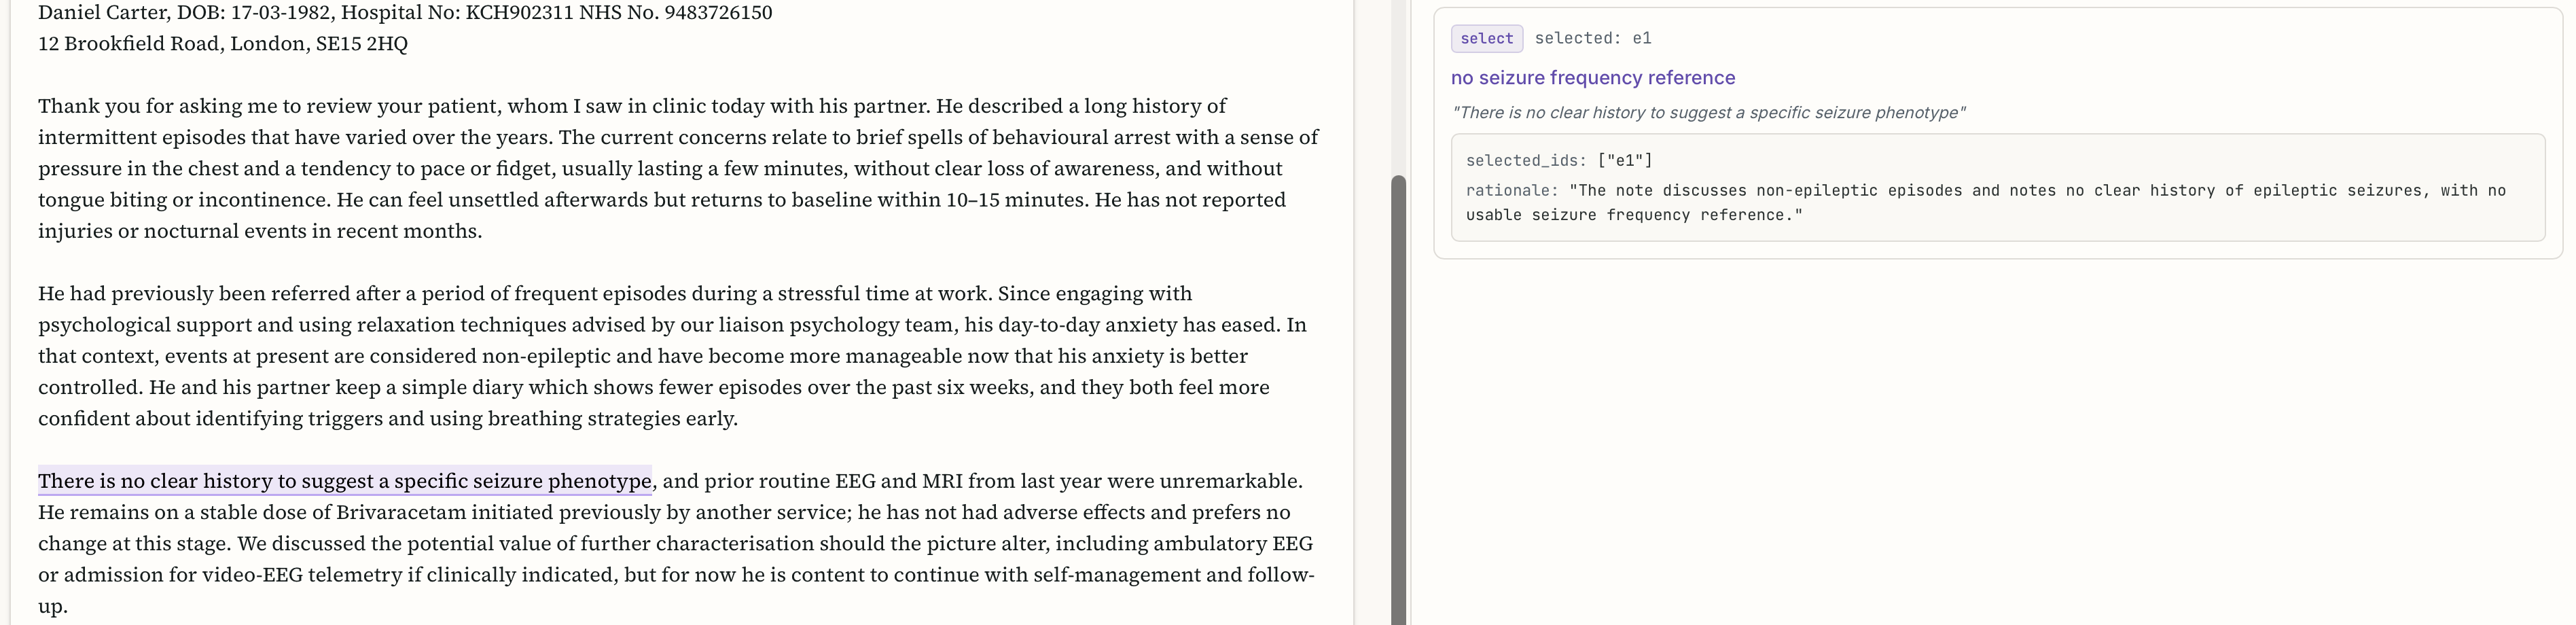
\includegraphics[width=\linewidth]{seizure_free_unknown}
        \caption{Seizure free → unknown error example. Gold-standard label: seizure free for multiple month. Model selected no seizure frequency reference (unknown).}
        \label{fig:frequent_unknown1}
    \end{subfigure}
    \caption{These examples illustrate the model choosing unknown when the gold-standard label was in the infrequent (a), frequent (b) and seizure free (c) categories. The rationale illustrates how the model interprets the ambiguous evidence and why it chooses unknown.}
    \label{fig:errors}
\end{figure*}

\subsection{Development Environment}

Experiments using local language models took place on a 
Dell XPS 16 9640 running Windows 11, with an Intel Core 
Ultra 9 185H, 32 GB RAM, and an NVIDIA GeForce RTX 
4070 Laptop GPU (8 GB VRAM). Ollama v0.32.15 was 
used to serve the models. Two models were run on local 
hardware (Qwen 3.8 27b, Gemma 4 26B). 

Experiments using hosted APIs were were run from a Mac 
mini M1 with 16 GB unified memory on macOS 26.5.2. API
calls were made directly to the provider (OpenAI, DeepSeek) 
or through model routers (OpenRouter, AI Gateway) Four 
hosted models were used (Gemini 3.7 Flash, GPT 5.6 Luna, 
Grok 4.6, DeepSeek v4 Flash). 

All models used a temperature of 0 except Luna, which only 
accepts a temperature of 1. An ablation was run on Gemini 
using a temperature of 1. All models used a thinking or effort 
level of 'low'. Ablations were run on Gemini using thinking
levels of medium and high. 

Python 3.14.4 was used to write the program. DSPy 3.2.1, 
Pydantic 2.13.4 and LiteLLM 1.87.1 were utilised as core
packages. DSPy was used to co-ordinate the model calls
and require structured JSON output. Pydantic was used
to validate the structured output conforms to the specified
schema. LiteLLM was used to deliver API calls to Ollama 
and the model routers.

\section{Discussion}

This paper shows that a combination of an LLM and rules
can extract an epilepsy patient's current seizure frequency 
burden as accurately as a fine-tuned LLM\cite{b2}. An LLM small 
enough to fit on a hospital's local servers can securely and 
reliably extract this information with no additional training 
or fine-tuning; a single LLM prompt designed to extract rich 
evidence followed by some rules to refine that evidence is 
just as accurate. This method requires significantly less 
computing power, data and expertise than training or 
fine-tuning an LLM, lowering barriers to adoption. Broader
use of automated clinical extraction pipelines can help 
expand the scope of real-world evidence (RWE) as an 
alternative to expensive clinical trials\cite{b2}.

The method is particularly effective at identifying patients
with the greatest disease burden; those with the most
frequent seizures. F1 scores of 0.92 for daily and 0.91
for more than weekly are substantially (0.2) higher than
prior methods\cite{b2}. This could be used in a few scenarios. 
It could be used in clinical care to flag patients with a seizure 
burden above a typical threshold for the clinician's attention. 
It could be used in cohort selection to identify patients to be 
enrolled in clinical trials for a new medication or to be 
recommended for surgery. It could be used to build a 
phenotypic profile of patients to be used in retrospective 
analyses to understand how these patients differ from the 
average. Finally, it could be used as an outcome variable in 
predictive models to identify patients likely to experience 
frequent seizures and recommend an early intervention\cite{b2}. 

The latest generation of LLMs are now capable enough 
to reliably populate rich schemas of facts and relations.
Past work in this area has typically tasked the LLM with 
producing a single answer in a fully normalised form\cite{b2}. 
This fails to leverage the rich semantic depth both in 
clinical narratives and within the model's capabilities.
Clinicians value unstructured narrative because it is 
more expressive; it allows them to convey their 
reasoning, uncertainty and vague impressions. These
nuanced observations are not only more honest
representations, they are more accurate and reliable\cite{b2}. 
LLMs are capable of preserving and reasoning
over those nuances, and preserving this richer evidence
chain can help build a more trustworthy, transparent 
system. In a clinical setting, a more explainable 
system is often a more useful system\cite{b2}.

There are a few limitations. Synthetic
data was used for all evaluations, and while past 
research has shown models fine-tuned on this dataset
generalise effectively to real world patient data\cite{b2},
the methods tested in this paper remain untested on 
real patient data. Past research has shown that rules
tuned on one corpus can generalise poorly to other 
corpuses, so the gains seen from rules in this method
may not generalise to other datasets. As this method 
was applied to a narrow task of seizure frequency 
extraction, future studies should evaluate whether 
it generalises to other common tasks in clinical IE. 
Alternatively, the modular pipeline applied to this 
seizure frequency task could be reconfigured to an
agentic pipeline, with LLMs deciding how to encode 
and select facts themselves in a more general 
framework. This kind of pipeline has shown promising 
results on clinical notes in oncology\cite{b2} and 
cardiology\cite{b2}.

\section{Conclusion}

\section*{References}

Please number citations consecutively within brackets \cite{b1}. The 
sentence punctuation follows the bracket \cite{b2}. 

\begin{thebibliography}{00}

\bibitem{b1} Wigglesworth et al., The incidence and prevalence of epilepsy in the United Kingdom 2013–2018: A retrospective cohort study of UK primary care data
\bibitem{b2} Fisher et al., Epilepsia 2014;55:475–482 (doi 10.1111/epi.12550)
\bibitem{b3} Y. Gan \emph{et al.}, ``Reproducible synthetic clinical letters for seizure frequency information extraction,'' arXiv:2603.11407, 2026.
\bibitem{b4} B. Fonferko-Shadrach \emph{et al.}, ``Annotation of epilepsy clinic letters for natural language processing,'' \emph{J. Biomed. Semantics}, vol.~15, no.~17, 2024.
\bibitem{b5} B. Holgate, J. Davies, S. Fang, J.~S. Winston, J.~T. Teo, and M.~P. Richardson, ``Fine-tuning LLMs to extract epilepsy seizure frequency data from health records,'' in \emph{Proc. 24th Workshop on Biomedical Language Processing (BioNLP)}, 2025, pp.~44--55.
\bibitem{b6} B.~M. Decker \emph{et al.}, ``Development of a natural language processing algorithm to extract seizure types and frequencies from the electronic health record,'' \emph{Seizure}, vol.~101, pp.~48--51, 2022.
\bibitem{b7} K. Xie \emph{et al.}, ``Extracting seizure frequency from epilepsy clinic notes: a machine reading approach to natural language processing,'' \emph{J. Amer. Med. Informat. Assoc.}, vol.~29, no.~5, pp.~873--881, 2022.
\bibitem{b8} B. Holgate \emph{et al.}, ``Extracting Epilepsy Patient Data with Llama 2'' 
\bibitem{b9} K. Xie, B. Litt, D. Roth, and C.~A. Ellis, ``Quantifying clinical outcome measures in patients with epilepsy using the electronic health record,'' in \emph{Proc. BioNLP Workshop}, 2022, pp.~369--375.
\bibitem{b10} M. Fernandes \emph{et al.},  ``Extracting Seizure Control Metrics from Clinic Notes of Patients with Epilepsy: a Natural Language Processing Approach'' 
\bibitem{b11} T. Brown \emph{et al.},  ``Language Models are Few-Shot Learners'' 
\bibitem{b12} M. Agrawal \emph{et al.},  ``Large Language Models are Few-Shot Clinical Information Extractors' 
\bibitem{b13} L. Cui \emph{et al.},  ``Complex epilepsy phenotype extraction from narrative clinical discharge summaries'' 
\bibitem{b14} S. Fu \emph{et al.}, ``Clinical concept extraction: A methodology review,'' \emph{J. Biomed. Informat.}, vol.~109, 2020, Art.~no.~103526.
\bibitem{b15} Y. Wang \emph{et al.}, ``Clinical information extraction applications: A literature review,'' \emph{J. Biomed. Informat.}, vol.~77, pp.~34--49, 2018.
\bibitem{b16} L. Chiticariu, Y. Li, and F. Reiss, ``Rule-based information extraction is dead! Long live rule-based information extraction systems!,'' in \emph{Proc. Conf. Empirical Methods in Natural Language Processing (EMNLP)}, 2013, pp.~827--832.
\bibitem{b17} Z. Yang \emph{et al.},  ``CLINES: Clinical LLM-based Information Extraction and Structuring Agent'' 
\bibitem{b18} J. Wang \emph{et al.},  ``Scaling Clinician-Grade Feature Generation from Clinical Notes with Multi-Agent Language Models'' 

\end{thebibliography}

\vspace{12pt}

\end{document}
